We can use network flow algorithm to find out the maximum number of edge-disjoint $s-t$ paths in a directed graph $G = (V, E)$.

The disjoint paths are paths which do not share edges. For example, there are $3$ edge-disjoint $s-t$ paths in the following figure.

\begin{figure}[H]
	\centering
	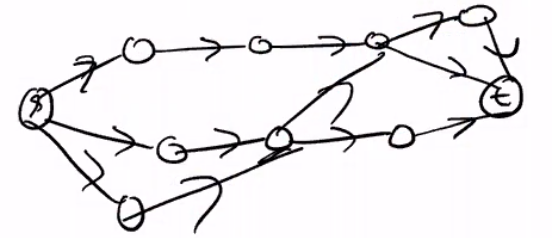
\includegraphics[width=0.5\textwidth]{fig/disjoint-path-eg.png}
\end{figure} 

How to find the largest number of such path? Set up flow network and set the capacity on each edge as 1.

\begin{theorem}
	Max flow value in this network equals max number of edge-disjoint paths from $s$ to $t$.
\end{theorem}

\begin{proof}
	It can be proved by proving two statements:
	\begin{itemize}
		\item If there are $k$ edge-disjoint paths, then there is a flow with value $k$.
		\item If max flow value is $k$, there are $k$ edge-disjoint paths.
	\end{itemize}

The first statement is easy to prove by conservation constrains. The capacity of each edge-disjoint path is $1$. Summing up $k$ of them give a flow of $k$.

For the second statement, suppose $k$ is an integer. Can assume max flow is integral. Every edge either carry 0 or 1 unit of flow. The idea is to find path one by one from the edge that carry non-zero flow.

Prove by induction on the number of edges carry non-zero flows.

\begin{itemize}
	\item Inductive state: the second statement is true for any graph with $n$ non-zero flow edges.
	\item Base case: one edge with non-zero flow. Then there is only one edge from $s$ going to $t$. The statement is obvious true since there is only one path.
	\item Inductive hypothesis: Assume that if there are $k$ edges with non-zero flow, then can find $k$ edge-disjoint paths.
	\item Inductive step: Consider a flow with $k+1$ edges with non-zero flow. 
	\begin{itemize}
		\item Case 1: Add one more edge and we reach $t$. So we find one $s-t$ path. Remove the edge from the graph. Remaining flow is a feasible flow on the remaining graph. Flow value is one less. Say original flow value was $F$. By induction, can find $F-1$ edge-disjoint path in remaining graph. Overall $F$ edge-disjoint paths.
		\item Case 2: If we get a cycle, can zero out flows on cycle. This preserve the flow value. But now the number of edges with non-zero flow $\le k$. Therefore, the theorem is true by inductive hypothesis.
	\end{itemize}
\end{itemize}
\end{proof}
\subsection{Duality Theorem}

Does the max-flow-min-cut theorem give us any additional insight here? Consider
max flow $f$, suppose there is a min-cut in the following plot. $F$ is the max flow value so $F = \#\text{ of edge-disjoint path}$. The capacity of min-cut is $F$.

\begin{figure}[H]
	\centering
	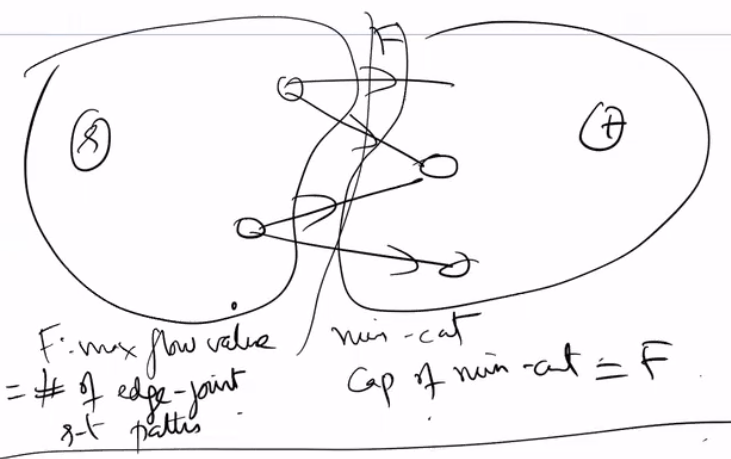
\includegraphics[width=0.5\textwidth]{fig/min-cut-eg.png}
\end{figure}

We know that the capacity of min-cut is the sum of the capacities of the forward edges. Since every edge has capacity 1, there must be $F$ forward edges for this min-cut.
 
\begin{theorem}
	(Menger's theorem 1927) If we remove $F$ edges we can disconnect $t$ from $s$. In a directed graph $G$ for any two vertices $s$, $t$, the max number of edge-disjoint $s-t$ path is equal to the minimum numbers of edges to remove to disconnect $t$ from $s$. 
\end{theorem}

\subsection{Further Extension: Undirected Graphs}
Can we find edge-disjoint paths in undirected graphs? It is easy convert undirected graph into a directed graph. So for any given $G$, $s$ and $t$, we can convert $G$ into $G'$ as a directed graph. Then put capacities as 1 on all the edges in $G'$. Then solve max flow as what we have done. 

But note that we may find edge-disjoint paths in directed graph, which may not be edge-disjoint in undirected. For example, there are two edge-disjoint path in the following graph but actually there are two edges share the same undirected edge. 

There is a quick fix for the problem, once you find the flow is carried by opposite edges then we can reduce at least one of them to zero. 
\begin{figure}[H]
	\centering
	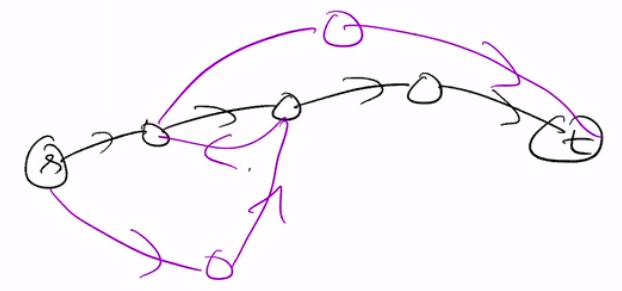
\includegraphics[width=0.5\textwidth]{fig/counter-example.png}
\end{figure}

\subsection{Further Extension: Multiple Sources and Sinks}
Think about a realistic situation: a company has many factories producing some object. Each factory can only produce a certain amount of product per day. So the supplies are available in different locations. Those produced product needs to be transported to certain distribution centers. Each distribution center has certain demands for the product. 

So what we have now is a network with multiple source and sink. Each factory is a source with certain level of supply of the product and each distribution center is a sink with certain need for the product.

Suppose each vertex $v$ has demand $d_v$. 
\begin{itemize}
	\item If $d_v > 0$, then $v$ has a demand $d_v$.
	\item If $d_v < 0$, then $v$ can supply $-d_v$.
\end{itemize}

Goal: Meet the ``demands'' at all vertices.

Necessary condition: \[\sum_{v: d_v > 0}|d_v| = \sum_{v:d_v < 0} |d_v| = D\]

Find feasible solution meaning capacity and demand conditions. Now the conservation constrain we normally have in flow has been replaced by demand conditions. We would not call the solution as a flow, instead, we call it a circulation since it does not satisfy conservation constrain anywhere.

If $v$ has demand $d_v$, \[\sum_{u: (u, v)\in E} - \sum_{u:(v, u)\in E} f(v, u) = d_v\]

The solution is simple. On the graph, have a super source and super sink in the graph $G$. For each supplier vertex with $d_v < 0$, connect an edge from the super source to it. For each distribution vertex with $d_v > 0$, connect an edge from the vertex to sink. Then the conservation constrain holds in the new graph and we can solve max-flow in the network. The max-flow is at most $D$. In fact, the max-flow needs to be $D$ in order to satisfy all demands.

If max-flow less than $D$, no feasible circulation. Otherwise, output is the answer.

\subsubsection{Further Extension: Capacities and Lower Bound Constrains}
Sometimes we would like to add some constrains at edge $e \in E$:
\begin{itemize}
	\item $f(e) \ge l(e)$
	\item $f(e) \le c(e)$
\end{itemize}

We can reduce this problem to a flow problem. First put lower bound amount of flow on each edge. Create a flow $f$, for each edge $e$, $f(e) = l(e)$. Doesn't satisfy conservation constrain.

Find a flow $f'$ to augment $f$. Final solution will be $f+f'$. $f'$ needs to re-establish conservation at all vertices besides $s$ and $t$. 

Let $d_v = \sum_{u} f(v, u) - \sum_u f(u, v)$. The capacity of each edge $e: c_e - l_e$. Find a circulation $f'$ in network with above demands and above capacities.

A feasible circulation solves the problem of finding a flow that satisfies both lower bound and capacity constrains.












